\newpage
\section*{SINGLE FILE LOCATION AND STRUCTURE}
% \parskip=0.3em
Files are an old and established mechanism used by applications to store and retrieve configuration, libraries, state, data etc. Most applications use files in their own unique manner and store files in various locations. This may lead to having files that are dispersed over different folders or hidden in system-folders of the Operating System. System administrators  want to be able to perform version control on the files.
\begin{center}
\ding{118} \ding{118} \ding{118}
\end{center}

\textbf{Having dispersed files causes system administrators to have difficulty in finding the files necessary for their tasks during the life cycle of an application.}\\

%forces
\begin{itemize}
\item Distributed Applications.\\
Many applications consist of different subsystems, which often require  subsystem-specific administration tasks. These subsystems are in many cases developed by different teams, resulting in dispersed groups of similar artifacts for each subsystem. This situation is well suited for developers as they can work in parallel. During deploy or system administration activities this can be a burden because of the
\item Hard-coded Locations.\\
It happens often that developers put the location of the configuration files in source code and provide no parameters or interface to influence this location. This means the path can only be changed by building and deploying a new version of the application. Running multiple instances of a program on a machine with different parameters is effectively blocked by this approach. Additionally it can pose security risks if the file location is in a privileged location such as \verb|C:\Program Files| for Windows based systems.
\item Pollution.\\
When a file of a module isn't used anymore it will easily remain in disuse and get overlooked which causes pollution of your hard disk.\\
%\item Non Human Readable Configuration Files.\\
%When an application provides a Graphical User Interface for configuring the application, it happens that such an application stores the captured configuration in a non human readable file. The disadvantage of this approach is that the system administrator can only see the configuration by starting the application and opening the dialogue to see the settings. This also blocks automation of deploy and install scripts and integration with automatic deploy tooling such as Puppet\footnote{\url{https://puppetlabs.com/}} or Chef\footnote{\url{http://www.opscode.com/chef/}}.
\end{itemize}

\begin{center}
\ding{118} \ding{118} \ding{118} 
\end{center}

\textbf{Therefore: Put all related files in one (hierarchical) location. Make the path of this location configurable.}\\

Analyze the files and folders of the application, group the files that logically belong together and should be at the same location e.g.: the binaries of a system, the configuration files and the data files. In the case of log files one should first consider to use {\sc Centralized System Logging}.

Ideally it should be a structure that is re-used across applications (see figure \ref{fig:singleFileLocationDiagram-01}) that are installed on the same server. This provides consistency for the system administrator, but also might help to overcome possible redundancies of files (e.g. keeping track of the language used). It furthermore serves as a clear guideline for the developers and could also be included in a reference architecture.

For reading the contents of configuration files {\sc Property Loader} and related patterns \cite{Wellhausen2010} can be used. 

\begin{figure}[h]
\centering
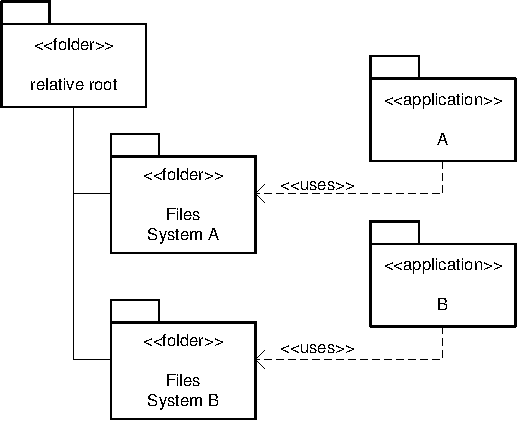
\includegraphics{patterns/singleFileLocationDiagram-01.pdf}
\caption{The hierarchical file structure}
\label{fig:singleFileLocationDiagram-01}
\end{figure}

The applications that do file access should not use the native File IO Libraries but should use a {\sc Facade} \cite{Gamma95} for accessing files (see figure \ref{fig:singleFileLocationDiagram-02}). This {\sc Facade} provides the basic file IO functionality and prohibits absolute path access. The {/sc Facade} is using a configurable absolute path that is the root of all file access. The relative paths branch from that root path.  This is best enforced in combination with a build server that checks which libraries are used from source code. The build should break when native File IO Libraries are used instead of the {\sc Facade}.

\begin{figure}[h!]
\centering
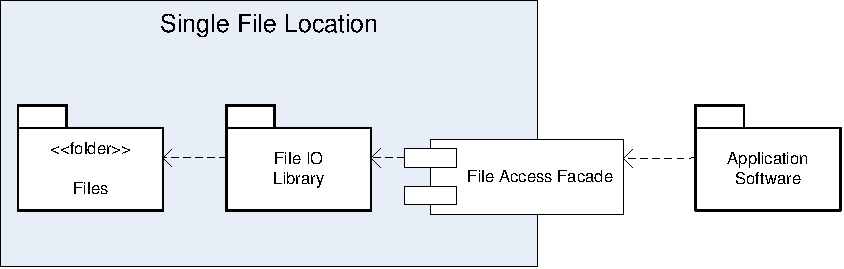
\includegraphics{patterns/singleFileLocationDiagram-02.pdf}
\caption{Main solution structure for file access using SINGLE FILE LOCATION}
\label{fig:singleFileLocationDiagram-02}
\end{figure}

Without using this pattern the files of applications will be dispersed over several distinct locations which makes it hard to maintain the application. 

If the folder structures are standardized across a development group, developers find it easier to navigate across an application and find the right files and folders.

Using SINGLE FILE LOCATION AND STRUCTURE is also more secure as this blocks access to vulnerable parts of the operating system as the implemented {\sc Facade} blocks access outside the root location. It is somewhat similar to a jailshell\footnote{Jailshell is a very limited shell that allows clients to logon to your server via SSH. It limits them to their home directories, keeping the rest of your files on your server from being viewed (\url{http://stackoverflow.com/tags/jail-shell/info).}} that prohibits users from wandering outside their home directories.

\textit{A nice example of the structure of SINGLE FILE LOCATION AND STRUCTURE without a {\sc Facade} is for instance found in the way Ruby on Rails\footnote{\url{http://rubyonrails.org/}} applications are structured. Every project starts with a pre-defined folder and file structure.}
 
%\begin{center}
%\ding{118} \ding{118} \ding{118} 
%\end{center}

%\textit{Rationale.}\\




